\chapter{Theoretical background}

\hspace{0.45cm} In this chapter, we are going to provides architectures and algorithms of related background in this thesis.
\section{Kalman filter}
\hspace{0.45cm}The Kalman filter is an algorithm allowing accurate inference in a linear dynamical system, 
where the state space of the latent variables is continuous and where all latent and observed variables have a Gaussian distribution.\cite{Kalman}\par
In the model of estimating state of pedestrian, trajectory changes with time as pedestrian change the current position to the next position based on
their current state, and the trajectory does not fluctuate too much. Moreover, the walking speed of an average person is 0.8m/s - 1.5m/s. Therefore,
the relative motion between the current position and the next position has a certain range. Finally, we can assume the model of estimating the state of pedestrian
is a dynamic linear model which is suitable to use Kalman filter to predict future state.

\begin{figure}[h!]
        \centering
        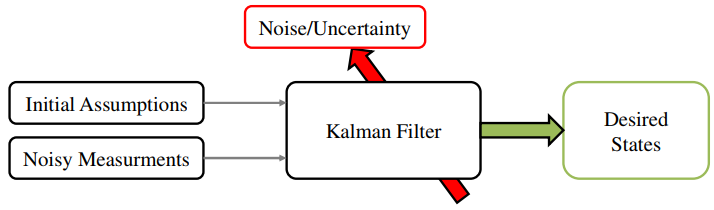
\includegraphics[width=\textwidth]{Chapters/Fig/kalman_dig.png}
        \caption{Diagram of Kalman filter}
        \label{fig:kalman_dig}
\end{figure}\par
Diagram of Kalman filter in fig.\ref{fig:kalman_dig}\cite{Kalman} shows the goal of the filter is to take in impefect 
information sort out the useful parts of interest, and to reduce the uncertainty or noise.\par
The dynamic linear model assumes that the state of a system that at a time $t$ derived from the prior state at the time $t-1$ 
defined by the following equation:
\begin{equation}
    \textbf{x}_t = \textbf{F}_t \textbf{x}_{t-1} + \textbf{B}_t \textbf{x}_t + \textbf{w}_t,
   \end{equation}\par
   where
   \begin{itemize}
       \item $\textbf{x}_t$ is the current state vector containing the parameters of interest of the system (e.g, position, velocity, accelerant..) at time t
       \item $\textbf{u}_t$ is the vector containing control inputs
       \item $\textbf{F}_t$ is the state transition matrix which applies the effect of each system state parameters at time $t-1$ on the system state at time $t$
       \item $\textbf{B}_t$ is the control input which applies the effect of each control input parameter in the control input vector $\textbf{u}_t$ on the state vector
       \item $\textbf{w}_t$ is the vector containing the process noise terms fro each parameter in the state vector.
   \end{itemize}
   
   \hspace{0.45cm}Measurements of the system is defined as follow:
   \begin{equation}
            \textbf{z}_t = \textbf{H}_t\textbf{x}_t + \textbf{v}_t,
   \end{equation}
   
   \hspace{0.45cm}where:
   \begin{itemize}
       \item $\textbf{z}_t$ is the vector of measurements
       \item $\textbf{H}_t$ is the transformation matrix that maps the state vector parameters into the measurement domain
       \item $\textbf{v}_t$ is the vector containing the measurement noise terms for each observation in the measurement vector
   \end{itemize}\par
   There is no direct observation of the true state $\textbf{x}_t$ of the system, and the Kalman filter provides an algorithm to estimate $\hat{\textbf{x}}_t$ using combination of models the system and noisy measurements. Hence, for now, the terms in interest in the state vector are distributed by Gaussian probability density functions (\acrshort{pdfs}) rather than discrete values. Gaussian \acrshort{pdfs} come up a co-variance matrix $\textbf{P}_t$ which has the diagonal containing the variances associated with the corresponding terms in the state vector and the remaining containing the co-variance between terms in the state vectors.\\
   In the prediction state, initial state estimate, $\hat{\textbf{x}}_0$ and $\textbf{P}_0$ are applied recursively at each time step, using a loop then the current state vector is predicted from the state dynamic equation defined as:
   \begin{center}
       $
           \hat{\textbf{x}}_{k|k-1} = \textbf{F}_{k-1}\hat{\textbf{x}}_{k-1} + \textbf{G}_{k-1}\textbf{u}_{k-1}, 
       $
   \end{center}
   \hspace{0.45cm}where:
   \begin{itemize}
       \item $\hat{\textbf{x}}_{k|k-1}$ is the predicted state vector
       \item $\hat{\textbf{x}}_{k}$ is the previous estimated state vector
       \item $\textbf{u}$ is the input vector
       \item $\textbf{F}$ and $\textbf{G}$ are the matrices defining the system dynamics
   \end{itemize}
   
   \hspace{0.45cm}Then we predict the state error co-variance matrix by following:
   \begin{equation}
             \textbf{P}_{k|k-1} = \textbf{F}_{k-1}\textbf{P}_{k-1}\textbf{F}^T_{k-1} + \textbf{Q}_{k-1}, 
   \end{equation}
   
   where:
   \begin{itemize}
       \item $\textbf{P}_{k|k-1}$ is the predicted state error co-variance matrix
       \item $\textbf{P}_{k-1}$ is the previous estimated state error co-variance matrix
       \item $\textbf{Q}$ is the process noise co-variance matrix.
   \end{itemize}\par
   One the predicted valued are obtained, the Kalman gain matrix, $\textbf{K}_k$ is calculated by the following function:
   \begin{equation}
                 \textbf{K}_k = \textbf{P}_{k|k-1} \textbf{H}^T_k(\textbf{H}_k\textbf{P}_{k|k-1} \textbf{H}^T_k + \textbf{R}_k)^{-1},  
   \end{equation}
   
   with $\textbf{R}$ is the measurement noise co-variance.\par
   The measurement update equations:
   \begin{itemize}
       \item The state vector is updated as:
           \begin{equation}
                         \hat{\textbf{x}}_k = \hat{\textbf{x}}_{k|k-1} + \textbf{K}_k(\textbf{z}_k - \textbf{H}_x\hat{\textbf{x}}_{k|k-1}), 
           \end{equation}
       \item The state error co-variance is updated by
           \begin{equation}
                         \textbf{P}_k = (\textbf{I} -  \textbf{K}_k\textbf{H}_k)\textbf{P}_{k|k-1}, 
           \end{equation}
   \end{itemize}



\pagebreak
\hspace{0.45cm}The workflow of Kalman filter is described in this the figure below:
\begin{figure}[h!]
    \centering
    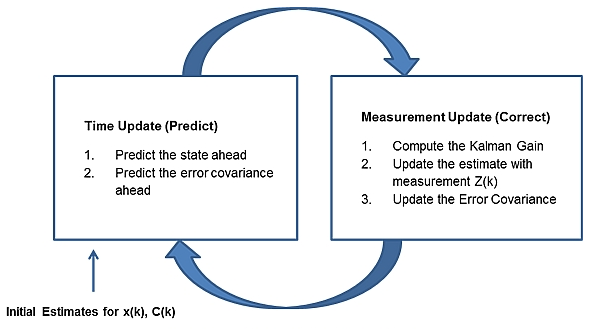
\includegraphics[scale=0.7]{Chapters/Fig/kal_dig_2.png}
    \caption{Workflow of Kalman filter}
    \label{fig:kalman_wf}
\end{figure}
\par
In fig.\ref{fig:kalman_wf}, two states "Predict" and "Correct" of Kalman filter 
occur continuously with the output of system in the time $t$ is the input of system in the time $t+1$, except the initial time $t_0$.
The efficient recursive functions minimize the mean of the squared error in order to provide an optimal status of the model. In several respects, the filter is very powerful: it supports estimates of past, present, and even future states, and it can do so even if the model system's precise nature is unknown.






\section{Object Detection}
\hspace{0.45cm}Object detection is one of the essential tasks in computer vision, the aim of object detection is that localize the instances and classify them in a
image. With the outburst of deep learning for decades, deep learning based approaches have not only achieved state-of-the-art performance but also
solved the problem in real time speed. In this section, we would like describe two prominent algorithms in object detections.
\subsection{Faster Region-based Convolutional Neural Network}
\hspace{0.45cm}Faster \acrshort{RCNN} is the third version of Region-based Convolutional Neural Network (\acrshort{RCNN}) family with some
improvements to increase the accuracy and the computational time. Instead of selective search to propose object region
for in two previous version \acrshort{RCNN} and Fast \acrshort{RCNN}, in Faster \acrshort{RCNN}, \cite{FrRCNN} proposed a network called \textit{Region Proposal Network} or \acrshort{RPN}. The comparison of three versions in RCNN
family is shown in the fig.\ref{fig:rcnn_family}\footnote{https://www.csdn.net/}
\begin{figure}[h!]
    \centering
    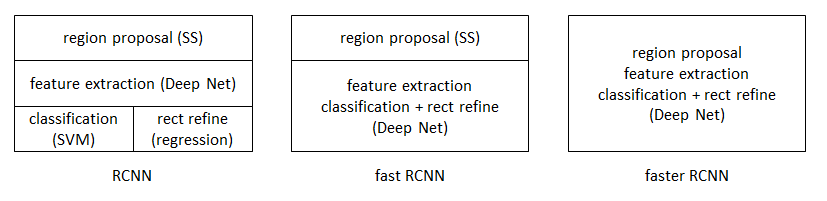
\includegraphics[width=\textwidth]{Chapters/Fig/rcnn-family.png}
    \caption{\acrshort{RCNN} object detection frameworks}
    \label{fig:rcnn_family}
\end{figure}
\subsubsection{The algorithm}
\begin{figure}[h!]
    \centering
    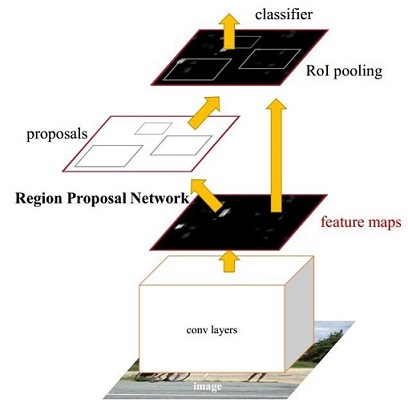
\includegraphics[width=0.7\textwidth]{Chapters/Fig/frrcnn.png}
    \caption{Faster \acrshort{RCNN} workflow diagram}
    \label{fig:frrcnn_workflow}
\end{figure}\par
The workflow diagram of Faster \acrshort{RCNN} is shown fig.\ref{fig:frrcnn_workflow}\cite{FrRCNN}.First, the input picture is cropped and the cropped picture is going through a pre-trained classification network or feature extraction network (VGG\cite{vgg}, Inception\cite{Szegedy_2015_CVPR}, ResNet\cite{He_2016_CVPR}) to obtain feature map corresponding to the images.\par
Then, take 9 candidate regions of interest(\acrshort{ROI}s) (3 different scales, 3 different aspect rations) on each anchor point on the feature map \cite{FrRCNN} , and map them to the original image according to the corresponding scale.\par
Third, these candidate \acrshort{ROI}s are then input into the \acrshort{RPN}, which would determine whether these \acrshort{ROI}s are foregroud or background and performs a preliminary regression (i.e. calculates the deviation of the bounding box between these foreground \acrshort{ROI}s and the ground truth) and then do \acrshort{NMS}\cite{SA}.\par
Next, perform ROI Pooling operations on these different sizes of \acrshort{ROI}s (map the the \acrshort{ROI}s to a specific size of feature map) and output a fixed size feature map.\par
Finally, it is input into a simple detection network, and then do classification and bounding box regression simultaneously.
\subsubsection{The architecture}
\begin{figure}[h!]
    \centering
    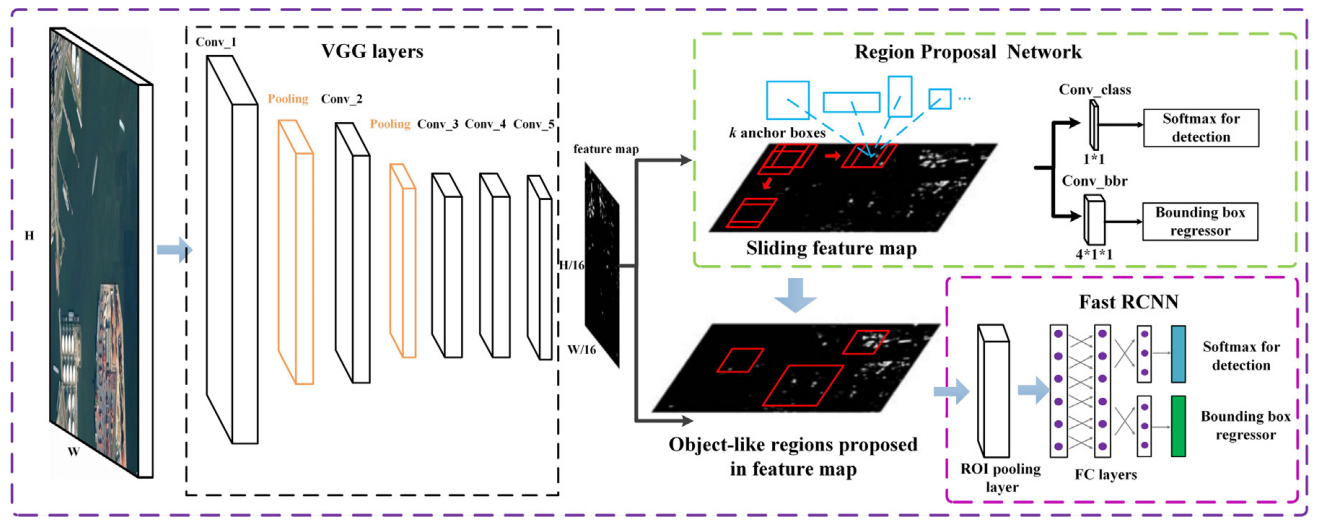
\includegraphics[width=0.85\textwidth]{Chapters/Fig/FrRCNN_arch.png}
    \caption{Faster \acrshort{RCNN} architecture}
    \label{fig:frrcnn_arc}
\end{figure}
Faster \acrshort{RCNN} adapts the architecture of two previous version of \acrshort{RCNN} family and improves the computation time by using Region Proposal Network instead of using selective search in order to choose \acrshort{ROI}s \cite{FrRCNN}. 
In other words, Faster \acrshort{RCNN} can be called \acrshort{RPN} + Fast \acrshort{RCNN}. For the feature extractor module. Faster \acrshort{RCNN} using VGG16\cite{vgg} pretrained on Image Net dataset \cite{FrRCNN}.\par
The Region Proposal Network (RPN) visualized in fig.\ref{fig:RPN}\footnote{https://www.researchgate.net} is efficiently to propose \acrshort{ROI}s of object in the image. 
\acrshort{RPN} has a classifier and a regressor. Classifier determines the probability of a proposal having the target object. Regression regresses the coordinates of the proposals.
\begin{figure}[h!]
    \centering
    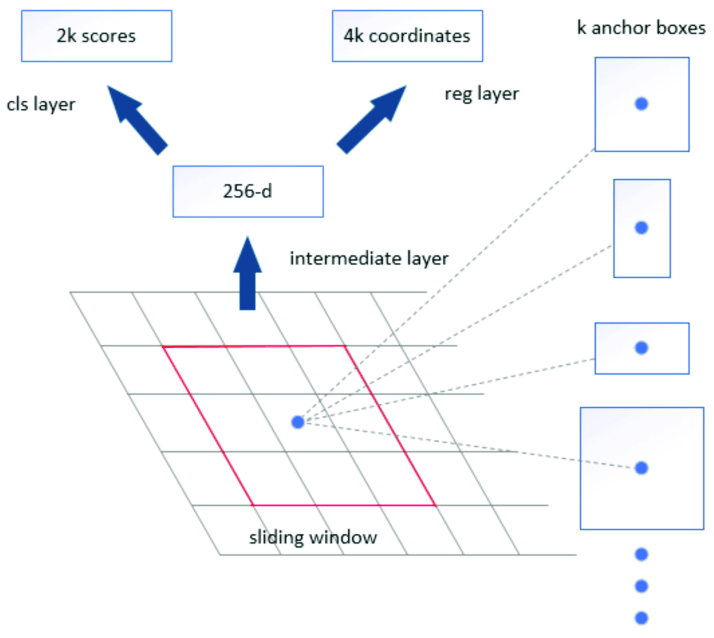
\includegraphics[width=0.6\textwidth]{Chapters/Fig/RPN_arc_1.png}
    \caption{Region Proposal Network mapping process}
    \label{fig:RPN}
\end{figure}
\par
It is a type of pooling layer which performs max pooling on inputs (here, convnet feature maps) 
of non-uniform sizes and produces a small feature map of fixed size (say 7x7)\cite{FrRCNN}. 
The choice of this fixed size is a network hyper-parameter and is predefined.
The main purpose of doing such a pooling is to speed up the training and test time and also to train the whole system from end-to-end (in a joint manner)\cite{FrRCNN}.

\subsection{YOLOv3}
\hspace{0.45cm}YOLOv3\cite{yolov3} is the third version of object detection algorithm in YOLO (You Only Look One) family. 
It increases the accuracy and improves the performance with many modifications than the previous version and is 
more ability of detecting small objects. The process flow of YOLOv3 is shown in fig.\ref{fig:yolov3_algo}\footnote{https://www.cyberailab.com}\par
\subsubsection{The algorithm}
\begin{figure}[h!]
    \centering
    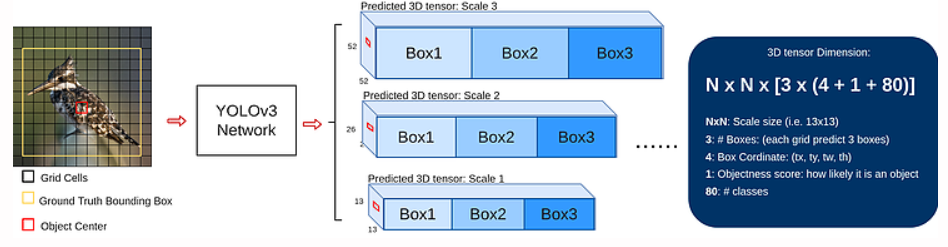
\includegraphics[width=\textwidth]{Chapters/Fig/yolo_algo.png}
    \caption{YOLOv3 Process Flow}
    \label{fig:yolov3_algo}
\end{figure}
\par
Firstly, YOLOv3\cite{yolov3} network predicts a 3D tensors with input images. The three scales processing is designed for detecting objects with various size 
in the input images. For example, with a scale of 13x13, the input image is divided into 13x13 grid cells and each grid cell corresponds to a 1x1x255 voxel inside
the output 3D tensor\cite{yolov3}. Concretely, 255 comes from (3 (anchor box/grid cell) x ( 4 (coordinates of predicted box) + 1 (object score) + 80 (class scores))).\par
Secondly, if the center point of the bounding box falls in a grid cell, this grid cell is responsible for evaluating the predicted bounding box of the object. For each grid cell, there are 3 anchor boxes assigned to it. The coordinates in the output tensor are the off-set values $t_x, t_y, t_w, t_h$, the applies the sigma function to constraint the offset values in range $[0,1]$. It makes the parametrization be easier to learn and the model is more stable\cite{Redmon_2017_CVPR}. \par
 In the fig.\ref{fig:bounding_box}\cite{Redmon_2017_CVPR}, $(c_x, c_y)$ is the offset from the top left corner of the image grid, $(p_x, p_h)$ is the predefined width and height of the corresponding anchor box, while $b_x,b_y,b_w,b_h$ is the respect to the normalized coordinates of the center and the size of the predicted box.
The predicted box which has the highest objectness score, and \acrshort{IoU} over the ground truth bounding box of the specfic class object is chosen.
\begin{figure}[h!]
    \centering
    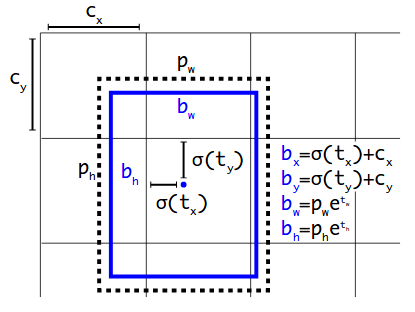
\includegraphics[scale=0.6]{Chapters/Fig/yolo_bounding_box.png}
    \caption{Predicted bounding box with dimensions priors and location prediction}
    \label{fig:bounding_box}
\end{figure}
\par
To choose the anchor boxes, the author uses the K-mean clustering algorithm to get 3 cluster means for each scale\cite{yolov3}. This results in 9 sizes chosen from 9 clusters, 3 for 3 different scale.
\subsubsection{The architecture}
\hspace{0.45cm}The architecture of YOLOv3 \cite{yolov3} is shown in fig.\ref{fig:yolo_arc}\footnote{https://www.cyberailab.com}.\par 
\begin{figure}[h!]
    \centering
    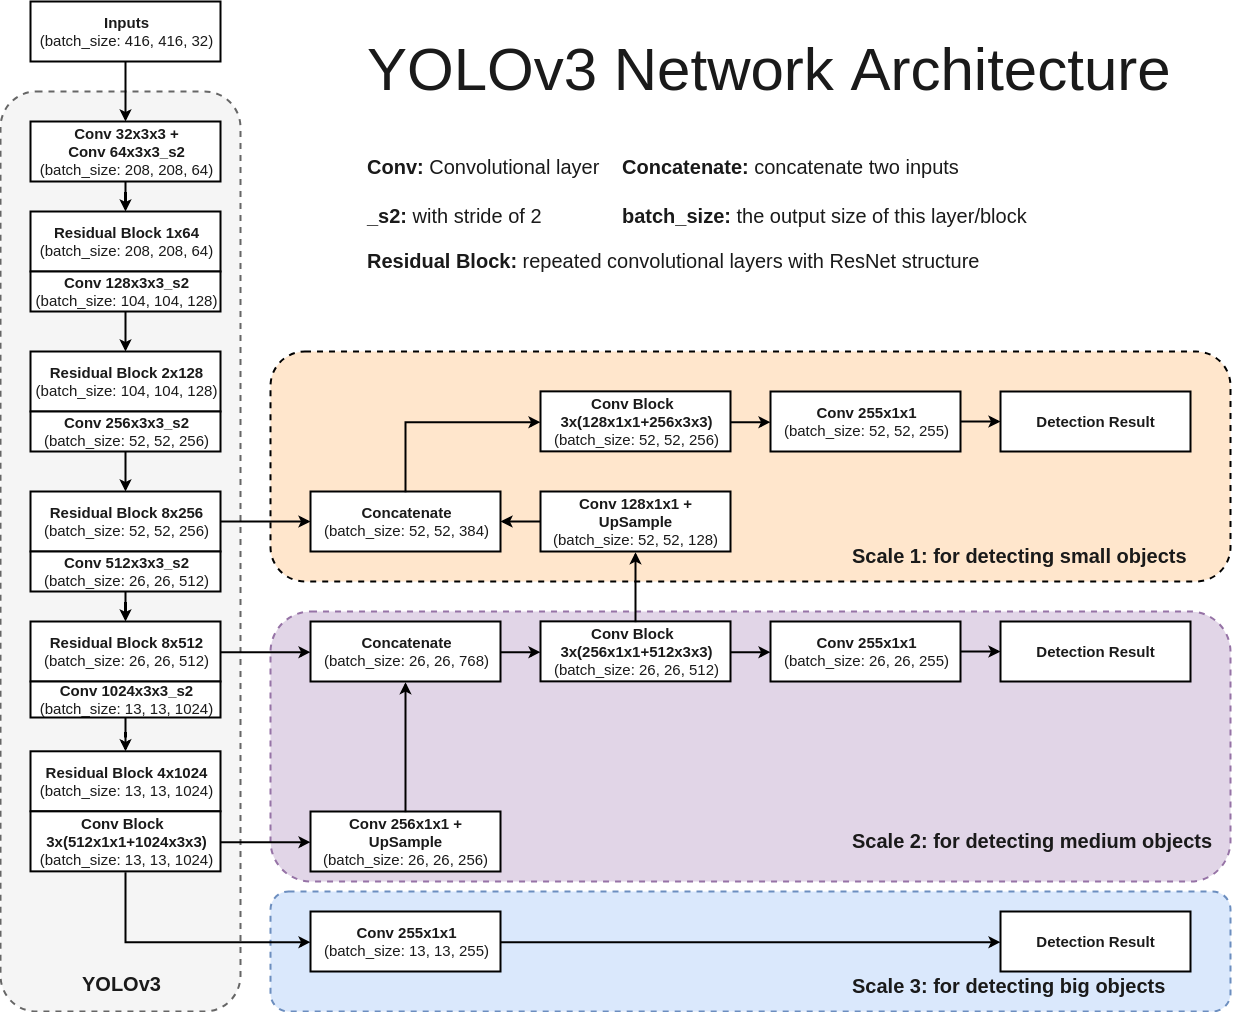
\includegraphics[scale=0.3]{Chapters/Fig/YOLOv3_architecture.png}
    \caption{YOLOv3 Network Architecture}
    \label{fig:yolo_arc}
\end{figure}

 Backbone network that was used to extract feature maps is Darknet-53\cite{yolov3}. 
 No fully-connected layer is used. This structure makes it possible to deal with images with
 any sizes. Also, no pooling layers are used\cite{yolov3}. Instead, a convolutional layer with stride 2 is used
 to down-sample the feature map, passing size-invariant feature forwardly.  In addition, a
 ResNet\cite{He_2016_CVPR}-alike structure (residual blocks) and FPN\cite{Lin_2017_CVPR}-alike (Feature Pyramid Network) structure is also
 a key to its accuracy improvement. \par There is no \textit{softmax} layer in YOLOv3, it is
 replaced by a 1x1 convolutional layer with logistic regression \cite{yolov3}. By using softmax, we have to
 assume that classes in the dataset are mutual independent while in some dataset, the labels are
 semantically similar \cite{yolov3}. Training with softmax might not let the network generalize the data
 distribution well. Instead, a logistic function is used to deal with multi-label classification \cite{yolov3}.

\section{Person Re-Identification}
\hspace{0.45cm}Person Re-identification is a task of detecting and precisely identifying a person from the a sequence images taken from different cameras or the same camera in different occasions. In this section, we would like to describe a creative approaches to solve this problem.
\subsection{Parameter-free Spatial Network for Person Re-Identification}

\subsubsection{The architecture}
\hspace{0.45cm} Global Average Pooling \cite{netinnet} or \acrshort{GAP} can focus on effective 
information for regression problems, 
but it may also cause some information to be lost\cite{SA}. 
Therefore, the author added spatial attention before the \acrshort{GAP} to improve the problem, 
as showing in fig.\ref{fig:sa_gap}\cite{SA}, where FCN represents the fully connected layer or \acrshort{FC} layer.\par
 \begin{figure}[h!]
     \centering
     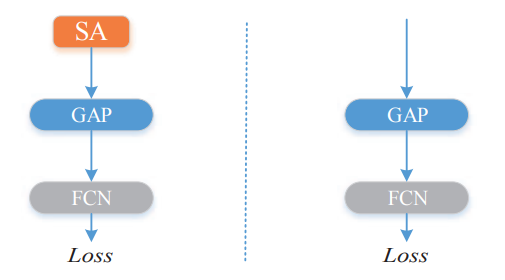
\includegraphics[scale=0.6]{Chapters/Fig/attention-sa-gap.PNG}
     \caption{Structure of a common classifier with \acrshort{GAP} is shown on the right, the modification on the left is that a spatial attention layer or \acrshort{SA} layer is inserted before \acrshort{GAP}}
     \label{fig:sa_gap}
 \end{figure}
The network architecture of parameter-free spatial attention network is shown in fig.\ref{fig:sa_arc}\cite{SA}.\par
\begin{figure}[h!]
    \centering
    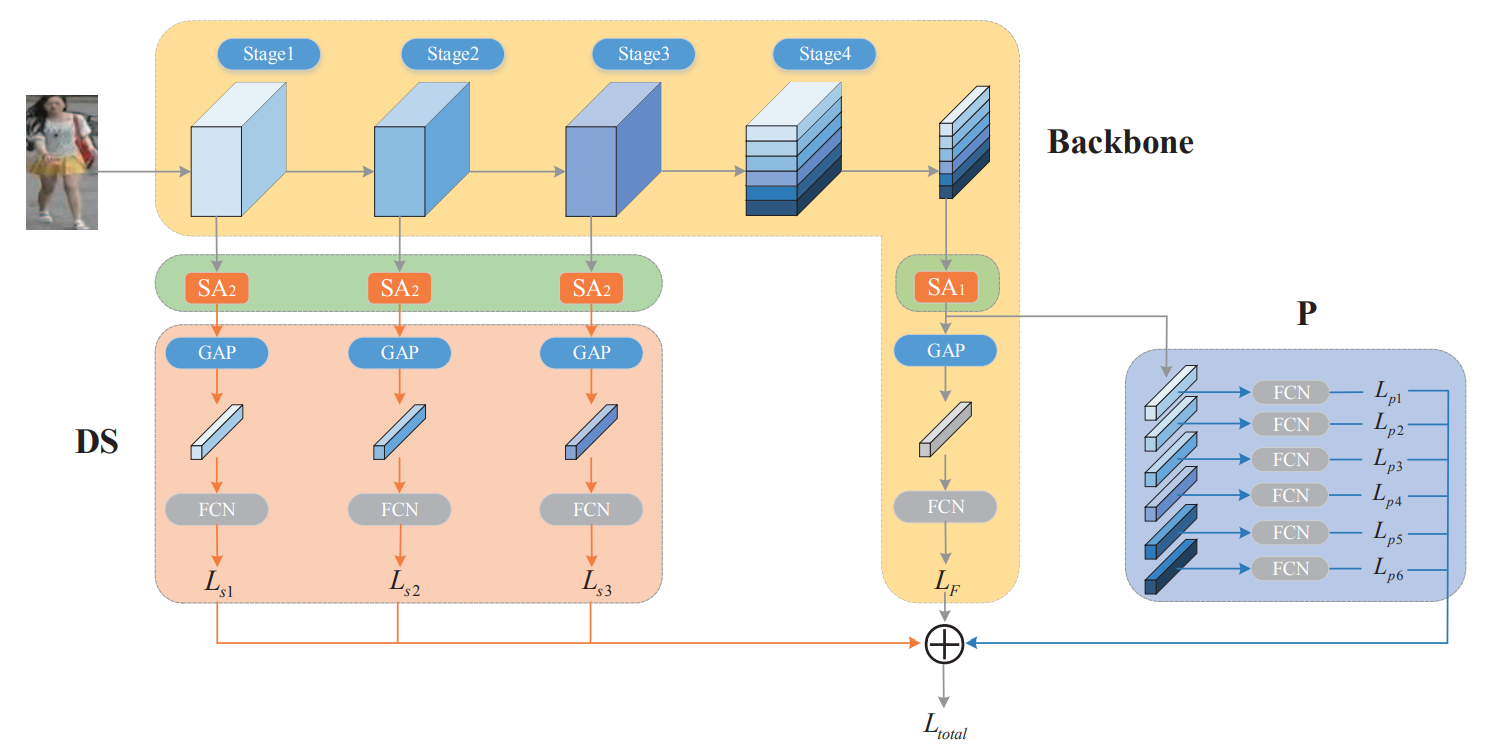
\includegraphics[width=\textwidth]{Chapters/Fig/attention_network.PNG}
    \caption{The network architecture}
    \label{fig:sa_arc}
\end{figure}
The yellow part is the backbone ResNet-50\cite{He_2016_CVPR}. The red part represents the deep supervision branches, for which the spatial attention layers (the left green part) are added before \acrshort{GAP}. The blue part denotes the part classifiers. Each part classifier produces a loss based on the part-level feature \cite{SA}. Note that the most right spatial attention part is not a part of the main model. It is only used in the ablation study \cite{SA}.\par
The input for every deeply supervised branch is a feature map $f$. The spatial attention layer first assigns different importance for different locations. The processed feature map is then fed into a \acrshort{GAP} layer followed by a fully-connected layer before computing the cross-entropy loss $l_{si}$\cite{SA}. Then the total loss is the summation over all deep supervision losses, six part losses and the loss from the backbone\cite{SA}.\par
During testing, all the deeply supervised branches and
part classifiers on top are dismissed. The backbone will then
be used as a feature extractor, which is applied to all the
query images and the images in gallery to obtain the features\cite{SA}. Then a standard information retrieval is performed
based on the Euclidean distance between these features\cite{SA}.
\subsubsection{Parameter-free Spatial Attention}
\hspace{0.45cm}As shown in fig.\ref{fig:sa}\cite{SA}, it is quite simple to compress the feature on the channel and use the method of directly adding the values of each channel to obtain a $H$x$W$x$1$ feature map, the reshape into a vector with size of $H$x$W$, then forward the vector through a softmax layer to obtain the weight of each element in the vector. Finally, we reshape vector of the weight to a volume with size of $H$x$W$x$1$ and concat with the original feature map.

\begin{figure}[h!]
    \centering
    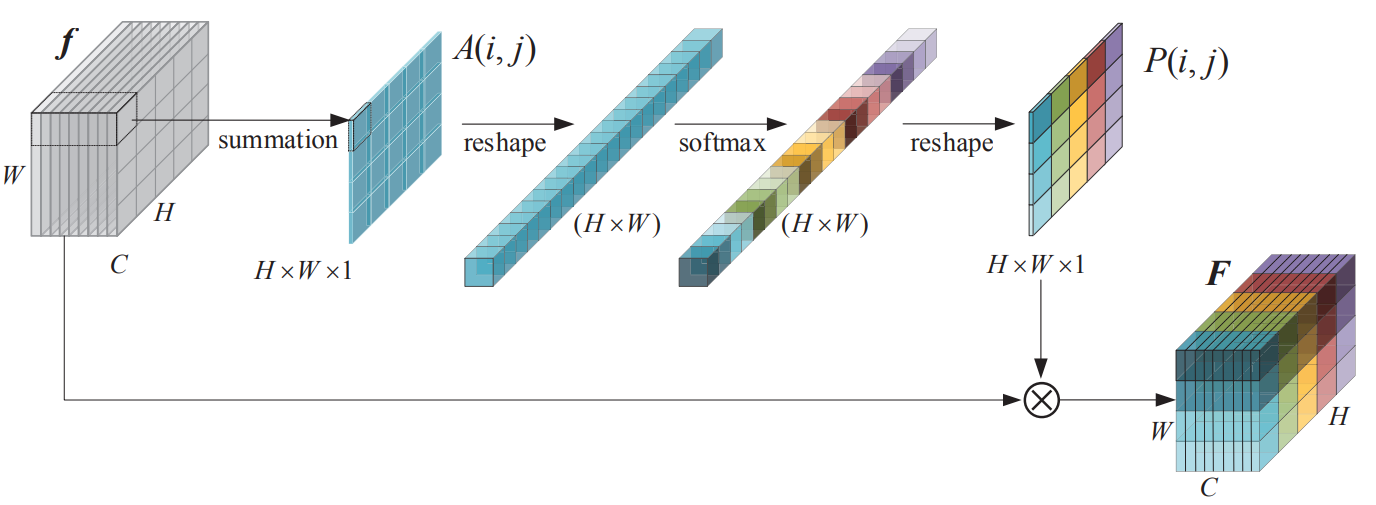
\includegraphics[scale=0.4]{Chapters/Fig/attention_sa.PNG}
    \caption{Parameter-free Spatial Attention Network Architecture}
    \label{fig:sa}
\end{figure}
\pagebreak
\section{Online pedestrian tracking methodologies}
\hspace{0.45cm} Online tracking-by-detection approaches usually operates the association the
detection of the current frame with a small number of the previous frames but not all the
information from the past. Otherwise, the performance of the method bases on the detection quality,
it means occlusions or miss detections can produce fragment trajectories, assign wrong
identifications. However, there are now many advanced techniques proposed to overcome this
problem,for example, Yi et al. \cite{MultiTracking} introduced a method using two-stage association with affinity features
calculated from detections obtained by using ACF detector to address these problems. However, this approach
only uses the detections for tracking process and does not take the advanced of large-scale person re-identification datasets.
On the other hand, Wojke et al. \cite{Wojke2017simple} proposed DeepSORT, a method that takes both detections and predictions 
from trackers with multi-stage matching stages and uses the deep learning-based features to perform online pedestrian tracking.
In this thesis, we would like to discuss more about DeepSORT\cite{Wojke2017simple} which we examine and then propose some architecture alterations to this approach.\par

DeepSORT or Simple online and realtime tracking with a deep association metric \cite{Wojke2017simple} is 
the a improvement of Simple online and realtime tracking \cite{sort} . DeepSORT\cite{Wojke2017simple} adapts effective parts from the previous version and integrates appearance information to improve the accuracy of SORT. All the computational complexity is placed 
into an offline pre-training stage where we learn a deep association metric on a large scale person re-identification dataset. \cite{Wojke2017simple}. The details of architectures
and algorithms of DeepSORT\cite{Wojke2017simple} will be further discussed in \autoref{Chap:3}





\section{Evaluation Metrics in MOT challenge}
\hspace{0.45cm}There has been a large number of metrics for quantitative evaluation of multiple target tracking has been proposed, however, due to the dataset for tracking problem in this work, the metrics in \cite{Milan2016MOT16AB} would be used and introduced in this section.
\subsection{Tracker-to-target assignment}
\hspace{0.45cm}There are two common essentials to quantifying the performance of a tracker. 
Firstly, to determine for each hypothesized output, whether it is a true positive (\acrshort{TP}
) that describes an actual (annotated) output or the output is a false positive (\acrshort{FP}),
 the decision is made by based on a defined distance measure $d$ which will be discussed later \cite{Milan2016MOT16AB}.
  If a target is not matched to any hypothesized output, it will be called a false negative (\acrshort{FN}). 
  In the other words, \acrshort{FP} denotes for number of false detections and \acrshort{FN} denotes for number of missed detections\cite{sort}. A result can be determined to be good if it has as few FPs and FNs as possible \cite{Milan2016MOT16AB}. 
  Then, to measure by the number of false alarm per frame or false positive per image in the object detection literature.\par
During the tracking process, it may happen that there are multiple outputs which covers the same target. 
The second prerequisite is then to establish the correspondence between all the annotated and hypothesized 
objects under the constraint that a true object should be recovered at most once, 
and that on hypothesis cannot account for more than one target \cite{Milan2016MOT16AB}. 
For the following, \cite{Milan2016MOT16AB} assumes that each ground truth trajectory has one unique start and end point. 
If a target leaves the \acrshort{FOV} and then reappears, the target would be assigned a new \acrshort{ID}. 
Therefore, the current metrics do not explicitly handle target re-identification \cite{Milan2016MOT16AB}. 
To be more accurate, if a ground truth object $i$ is matched to hypothesis $j$ at time $t-1$ and the distance between $i$ and $j$ at 
frame $t$ is under the threshold distance, the correspondence between $i$ and $j$ still 
remain even if there exists a hypothesis $k$ that is closer distance to ground truth $i$. 
An identity switch is counted if a ground truth target $i$ is matched to a track $j$ and the last known assignment was $k\neq j$ \cite{Milan2016MOT16AB}.\par
\begin{figure}[h!]
    \centering
    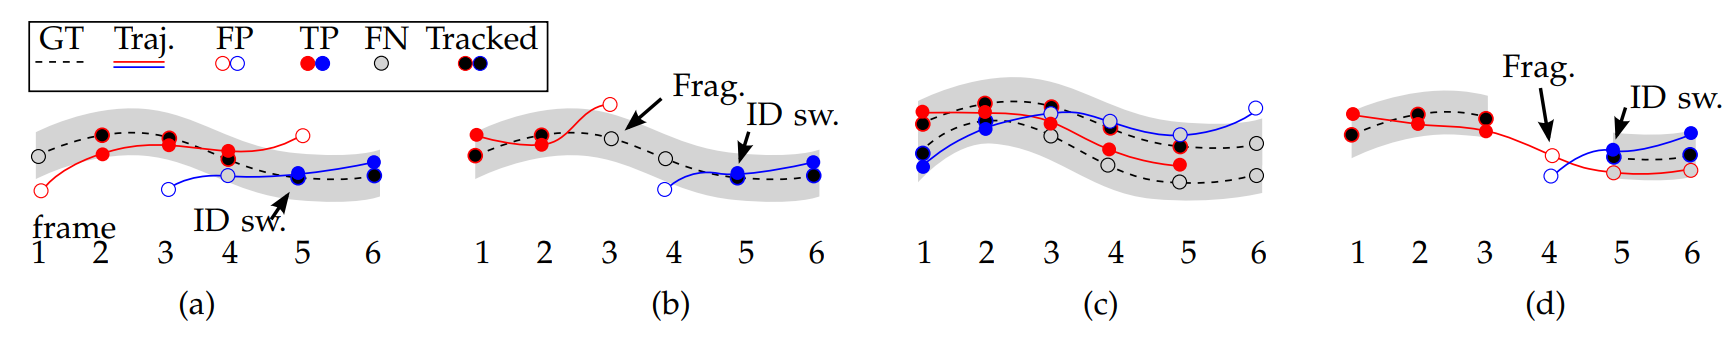
\includegraphics[width=\textwidth]{Chapters/Fig/id_switch_mot.png}
    \caption{Four cases illustrating tracker-to-target assignments}
    \label{fig:ids_mot}
\end{figure}
Fig.\ref{fig:ids_mot}\cite{Milan2016MOT16AB} illustrated cases that cause \acrshort{ID} switches in the tracking evaluation process. 
\cite{Milan2016MOT16AB} plots ground truth trajectories with dashed curved, and the tracker output with solid ones, 
where the color represents a unique target \acrshort{ID}. The grey areas indicate the matching threshold (see next section). Each
true target that has been successfully recovered in one particular frame is represented with a filled black dot with a stroke color corresponding to its matched hypothesis.\par 
To be more detailed\cite{Milan2016MOT16AB} , (a) An \acrshort{ID} switch occurs when the mapping switches from the previously assigned red track to the blue one. (b) A track fragmentation is counted in frame 3 because the target is tracked in frames 1-2, then interrupts, and then reacquires its ‘tracked’ status at a later point. A new (blue) track hypothesis also causes an \acrshort{ID} switch at this point. (c) Although the tracking results are reasonably good, an optimal single-frame assignment in frame 1 is propagated through the sequence, causing 5 missed targets (\acrshort{FN}) and 4 false positives (\acrshort{FP}). Note that no fragmentation is counted in frames 3 and 6 because tracking of those targets is not resumed at a later point. (d) A degenerate case illustrating that target re-identification is not handled correctly. An interrupted ground truth trajectory will typically cause a fragmentation.
\subsection{Distance measure}
\hspace{0.45cm}Because the presentation of objects in the image plane is the bounding box, to measure the similarity, \cite{Milan2016MOT16AB} employ intersection over union or \acrshort{IoU} with the threshold $t_d$ is set to 0.5 or 50\%.
\subsection{Multiple Object Tracking Accuracy}
The multiple object tracking accuracy or \acrshort{MOTA} is the most widely used metric to evaluate a tracker's performance because of its expressiveness as it combines three 
sources of the errors defined above:
\begin{equation}
    \text{MOTA} = 1 - \frac{\sum_t(\text{FN}_t + \text{FP}_t + \text{IDSW}_t)}{\sum_t\text{GT}_t}
\end{equation}
\subsection{Multiple Objects Tracking Precision}
\hspace{0.45cm}Multiple objects tracking precision or \acrshort{MOTP} is a measure of localization precision, 
not to be confused with positive predictive value or relevance in the context of precision/recall curves used in object detection\cite{Milan2016MOT16AB}. \acrshort{MOTP} 
is the average dissimilarity between all true positives and their corresponding ground truth targets, the \acrshort{MOTP} is defined as:
\begin{equation}
    \text{MOTP} = \frac{\sum_{t,i}d_{t,i}}{\sum_t c_t}
\end{equation}
where $c_t$ is the number of matches in frame $t$ and $d_{t,i}$ is the bounding box overlap of target $i$ with its assigned ground truth object.
\subsection{Tracking quality measures}
\hspace{0.45cm}Each ground truth trajectory can be classified as mostly tracked (\acrshort{MT}), partially tracked (\acrshort{PT}), and mostly lost
(\acrshort{ML}). This is done based on how much of the trajectory is recovered by the tracking algorithm. A target is mostly
tracked if it is successfully tracked for at least 80\% of its life span \cite{Milan2016MOT16AB}. If a track is only recovered for less than 20\% of its total length, it is said to be mostly lost (\acrshort{ML}). All other
tracks are partially tracked. A higher number of \acrshort{MT} and fewer \acrshort{ML} is desirable.

